\section{Further Improvements}


\begin{itemize}
    \item You can modify the calibration factor $(calibration\_factor)$ to adjust the scale according to your specific load cell and measurement requirements.
    \item By using the purple hx711, that has bigger and more separated tracks, it is possible to benefit from an improvement in terms of precision, since the entity of the disturbances is smaller.
    
    \begin{figure}[H]
    \centering
    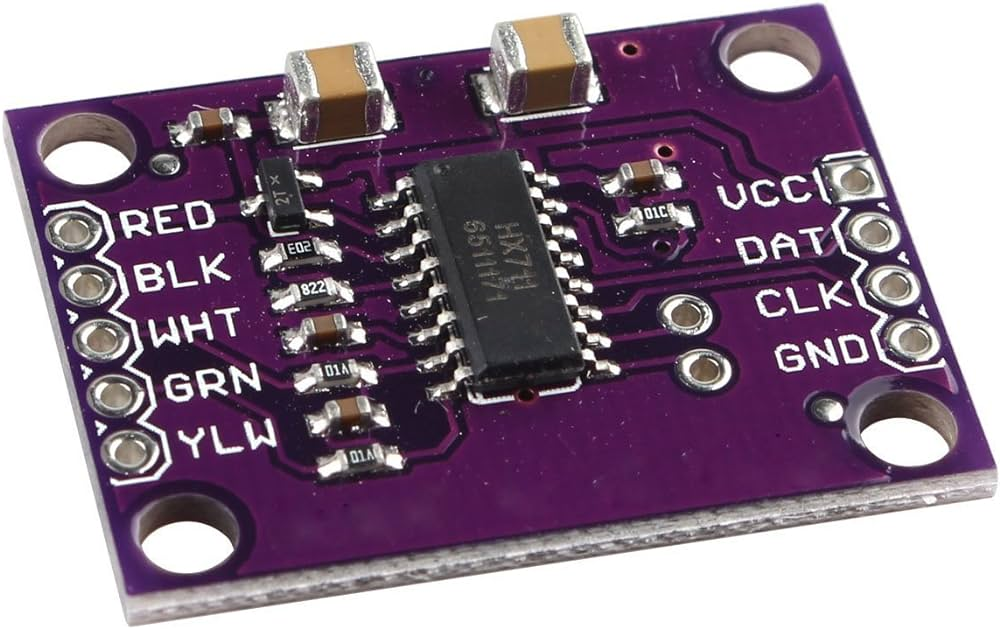
\includegraphics[width=0.5\linewidth, height=6cm]{medias/parts/purple_hx711.jpg}
    \caption{Purple HX711}
    \label{fig:purplehx711}
    \end{figure}
    \noindent

    \item The program can be extended to support different measurement units by adding appropriate conversions and displaying the result in the desired unit on the LCD screen.
    \item Error handling and validation can be implemented to handle exceptional cases, such as when the load cell is not connected or when the measurements are out of range, making them block the execution of the entire program.
    \item You can compile this code to run also on other boards that are better for 3D printed cases (actually tested on Arduino Uno, ESP8266)
\end{itemize}

